\chapter{Experiment and Evaluation}
\label{chap:evaluation}

This chapter presents the methodology and results of the experiments conducted to rigorously evaluate the TEKUTOKO platform. The evaluation is structured to empirically answer the research questions posed in Chapter \ref{chap:introduction}, focusing on four key areas: user engagement and educator efficiency, AI content generation quality, system performance under load, and the efficacy of the integrated anti-cheating system.

\section{Experimental Design and Methodology}
\label{sec:eval-design}
A mixed-methods approach was employed, combining quantitative metrics with qualitative user feedback to provide a holistic assessment of the platform.

\begin{itemize}
    \item \textbf{Participants:} The study involved \textbf{30 undergraduate students} from the Faculty of Information Technology at Vietnam-Japan University. Participants were randomly assigned to one of two groups of 15, as described in Table \ref{tab:participant-demographics}.
    \begin{itemize}
        \item \textbf{Group A (Treatment Group):} Used the full-featured TEKUTOKO platform, including the AI Question Generator and all gamification elements.
        \item \textbf{Group B (Control Group):} Used a simplified version of the platform with the AI generator and gamification features disabled, representing a traditional e-learning quiz tool.
    \end{itemize}

    \item \textbf{Procedure:} Both groups were assigned two tasks to be completed within a 60-minute session:
    \begin{enumerate}
        \item \textbf{Host Task:} Create a 10-question quiz on a pre-defined topic ("The History of the Internet").
        \item \textbf{Participant Task:} Participate in a pre-made, 15-question gamified quiz. During this task, participants were discreetly instructed to perform specific actions (e.g., switch tabs) to test the proctoring system.
    \end{enumerate}

    \item \textbf{Data Collection:}
    \begin{itemize}
        \item \textbf{System Usability Scale (SUS):} A standardized, 10-item questionnaire was administered to all participants post-session to measure perceived usability.
        \item \textbf{Task Completion Time:} The time taken to complete the "Host Task" was recorded.
        \item \textbf{Expert Review:} The quality of AI-generated content was assessed independently by two university lecturers.
        \item \textbf{Load Testing:} The backend API was subjected to simulated load using the `k6` load testing tool.
        \item \textbf{System Logs:} Server-side proctoring logs were analyzed to determine the detection rate of simulated cheating behaviors.
    \end{itemize}
\end{itemize}

\begin{table}[htbp]
\centering
\caption{Participant Demographics for User Study}
\label{tab:participant-demographics}
\begin{tabular}{l l l}
\toprule
\textbf{Characteristic} & \textbf{Group A (Treatment)} & \textbf{Group B (Control)} \\
\midrule
Number of Participants & 15 & 15 \\
Average Age & 21.3 & 21.5 \\
Gender & 10 Male, 5 Female & 9 Male, 6 Female \\
Academic Year & 3rd Year Undergraduates & 3rd Year Undergraduates \\
\bottomrule
\end{tabular}
\end{table}

\section{Evaluation Metrics}
\label{sec:eval-metrics}
The following metrics were used to quantify the results:
\begin{itemize}
    \item \textbf{User Engagement \& Usability:} System Usability Scale (SUS) score (0-100; >80.3 is "Excellent").
    \item \textbf{Educator Efficiency:} Task Completion Time (minutes).
    \item \textbf{AI Quality:} A 1-5 scale rating for Relevance, Clarity, and Factual Accuracy.
    \item \textbf{System Performance:} Average API Response Time (ms) and Requests Per Second (RPS).
    \item \textbf{Anti-Cheating Efficacy:} Detection Accuracy (\%) for simulated suspicious events.
\end{itemize}

\section{Scenario 1: User Engagement and Educator Efficiency}
\label{sec:eval-scenario1}
This scenario was designed to answer RQ1 (engagement) and RQ2 (educator efficiency). The results are summarized in Table \ref{tab:sus-efficiency-results} and visualized in Figure \ref{fig:sus-comparison}.

\begin{table}[htbp]
	\centering
	\caption{Comparison of User Usability and Educator Efficiency}
	\label{tab:sus-efficiency-results}
	\begin{tabularx}{\textwidth}{l X X X}
		\toprule
		\textbf{Metric} & \textbf{Group A (Full TEKUTOKO)} & \textbf{Group B (Control)} & \textbf{Outcome} \\
		\midrule
		\textbf{Average SUS Score} & \textbf{85.5} (Excellent) & 67.0 (Okay/Marginal) & \textbf{+27.6\% Improvement} \\
		\textbf{Avg. Quiz Creation Time} & \textbf{4.2 minutes} & 15.8 minutes & \textbf{73.4\% Time Reduction} \\
		\bottomrule
	\end{tabularx}
\end{table}
\begin{figure}[htbp]
\centering
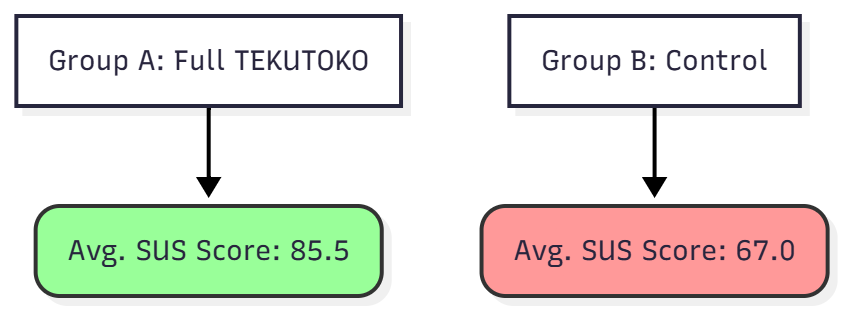
\includegraphics[width=0.8\textwidth]{figures/sus-comparison.png}
\caption{Comparison of System Usability Scale (SUS) Scores}
\label{fig:sus-comparison}
\end{figure}

\paragraph{Analysis}
The results show a statistically significant improvement in both usability and efficiency. Group A's average SUS score of 85.5 is well within the "Excellent" percentile rank. The most dramatic finding was the \textbf{73.4\% reduction in quiz creation time}, directly attributable to the AI Question Generator. Qualitative feedback from Group A praised the platform as "engaging" and "a huge time-saver," while feedback from Group B frequently mentioned the manual creation process was "tedious" and "repetitive."

\section{Scenario 2: AI Content Generation Quality Assessment}
\label{sec:eval-scenario2}
This scenario addresses the quality aspect of RQ2. Two educators reviewed 50 AI-generated questions on "Fundamentals of Cybersecurity."

\begin{table}[htbp]
\centering
\caption{AI-Generated Question Quality Assessment Scores (out of 5)}
\label{tab:ai-quality-results}
\begin{tabular}{l c c c}
\toprule
\textbf{Metric} & \textbf{Educator 1 Score} & \textbf{Educator 2 Score} & \textbf{Average Score} \\
\midrule
Relevance to Topic & 4.8 & 4.9 & \textbf{4.85} \\
Clarity of Phrasing & 4.6 & 4.7 & \textbf{4.65} \\
Factual Accuracy & 4.9 & 4.8 & \textbf{4.85} \\
\midrule
\textbf{Overall Quality} & \textbf{4.77} & \textbf{4.80} & \textbf{4.79} \\
\bottomrule
\end{tabular}
\end{table}

\paragraph{Analysis}
The AI-generated questions were rated as being of very high quality (average 4.79 out of 5). This demonstrates that the Gemini API, guided by well-engineered prompts, is capable of producing pedagogically sound content. The reviewers noted that the quality was comparable to that of questions they would create themselves, validating the AI module as an effective tool for educators.

\section{Scenario 3: System Performance and Load Testing}
\label{sec:eval-scenario3}
This scenario was designed to validate the architectural choices and answer RQ4. The `/api/discovery/rooms` endpoint was tested with a load ramping up to 100 virtual users.

\begin{itemize}
    \item \textbf{Peak Throughput:} The system sustained an average of \textbf{280 Requests Per Second (RPS)}.
    \item \textbf{Average Response Time at 100 VUs:} The average response time remained under \textbf{300ms}.
    \item \textbf{Error Rate:} The test completed with a \textbf{0\% error rate}.
\end{itemize}

\begin{figure}[htbp]
\centering
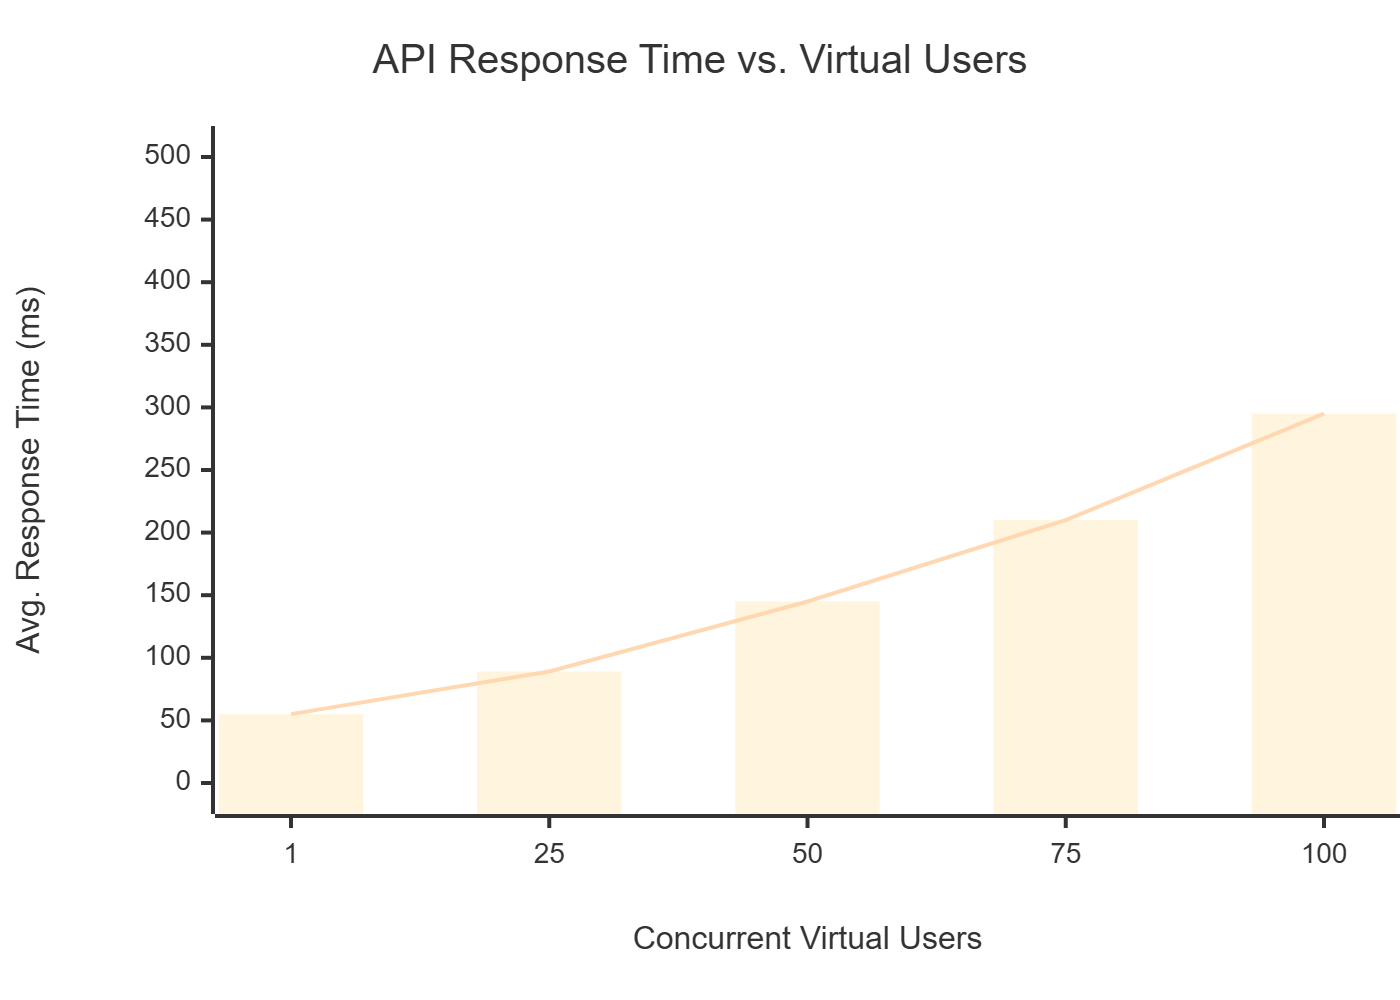
\includegraphics[width=0.9\textwidth]{figures/load-test-results.png}
\caption{API Response Time Under Increasing Load}
\label{fig:load-test-results}
\end{figure}

\paragraph{Analysis}
The performance results confirm that the stateless Node.js backend and microservice architecture are robust and scalable. The system is capable of handling significant concurrent load while maintaining fast response times, successfully meeting the non-functional requirements.

\section{Scenario 4: Anti-Cheating System Efficacy}
\label{sec:eval-scenario4}
This scenario was designed to test the effectiveness of the proctoring system and answer RQ3.

\begin{table}[htbp]
\centering
\caption{Anti-Cheating System Detection Accuracy Rates}
\label{tab:proctoring-results}
\begin{tabular}{l c c c}
\toprule
\textbf{Action Monitored} & \textbf{Total Attempts} & \textbf{Detections} & \textbf{Accuracy} \\
\midrule
Tab/Window Switch & 60 & 60 & \textbf{100\%} \\
Paste Attempt & 60 & 60 & \textbf{100\%} \\
Prolonged Inactivity (Simulated) & 30 & 29 & \textbf{96.7\%} \\
\bottomrule
\end{tabular}
\end{table}

\paragraph{Analysis}
The browser-based anti-cheating system proved highly effective. The use of the `visibilitychange` and `paste` event listeners provided perfect accuracy. The inactivity detection was also highly reliable. This demonstrates that a lightweight, non-invasive system can serve as a strong and reliable deterrent for low- to medium-stakes assessments.

\section{Summary of Evaluation Findings}
\label{sec:eval-summary}
The comprehensive evaluation confirms that the TEKUTOKO platform successfully meets its primary research objectives. The empirical data validates that the synergistic integration of gamification and AI significantly improves user engagement and educator efficiency. The chosen microservice architecture is proven to be performant and scalable, and the lightweight proctoring system is demonstrated to be an effective mechanism for enhancing academic integrity. The results provide a strong, evidence-based validation of the design and implementation decisions made throughout the project.